%!TEX root = ../main.tex
\vspace{-0.5em}
\subsection{Coreset Size Selection of \ours}
\label{exp:sec:end2end}

% \begin{figure}
% 	\centering
% 	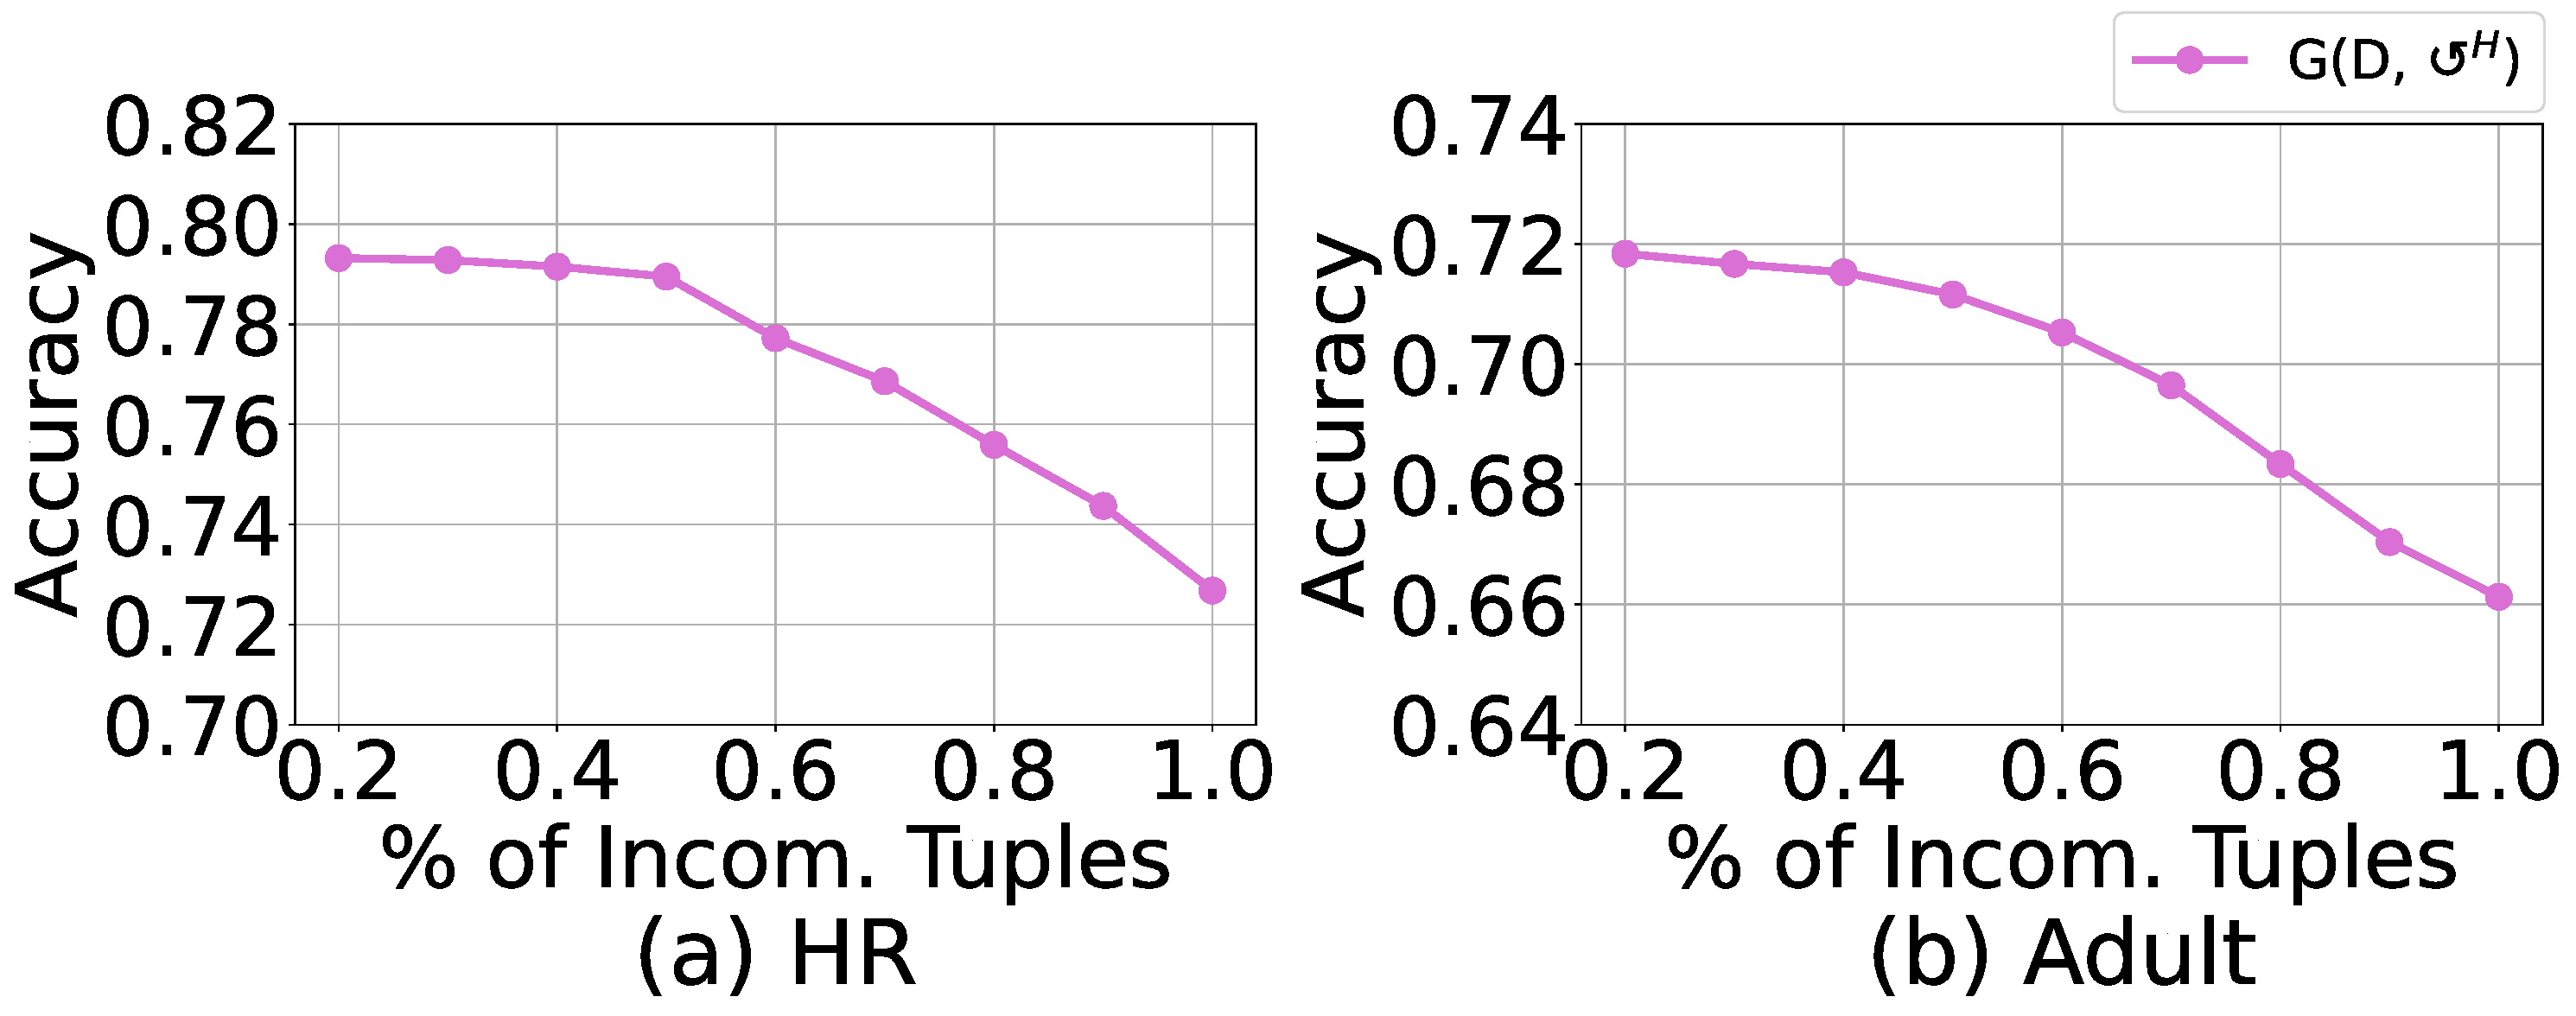
\includegraphics[width=0.5\textwidth]{figs/missingrate_all}
% %	\vspace{-1em}
% 	\caption{Varying missing tuple rate.}
% 	\label{fig:vary_misstuple_all}
% %	\vspace{-1em}
% \end{figure}

% \begin{figure}
% 	\centering
% 	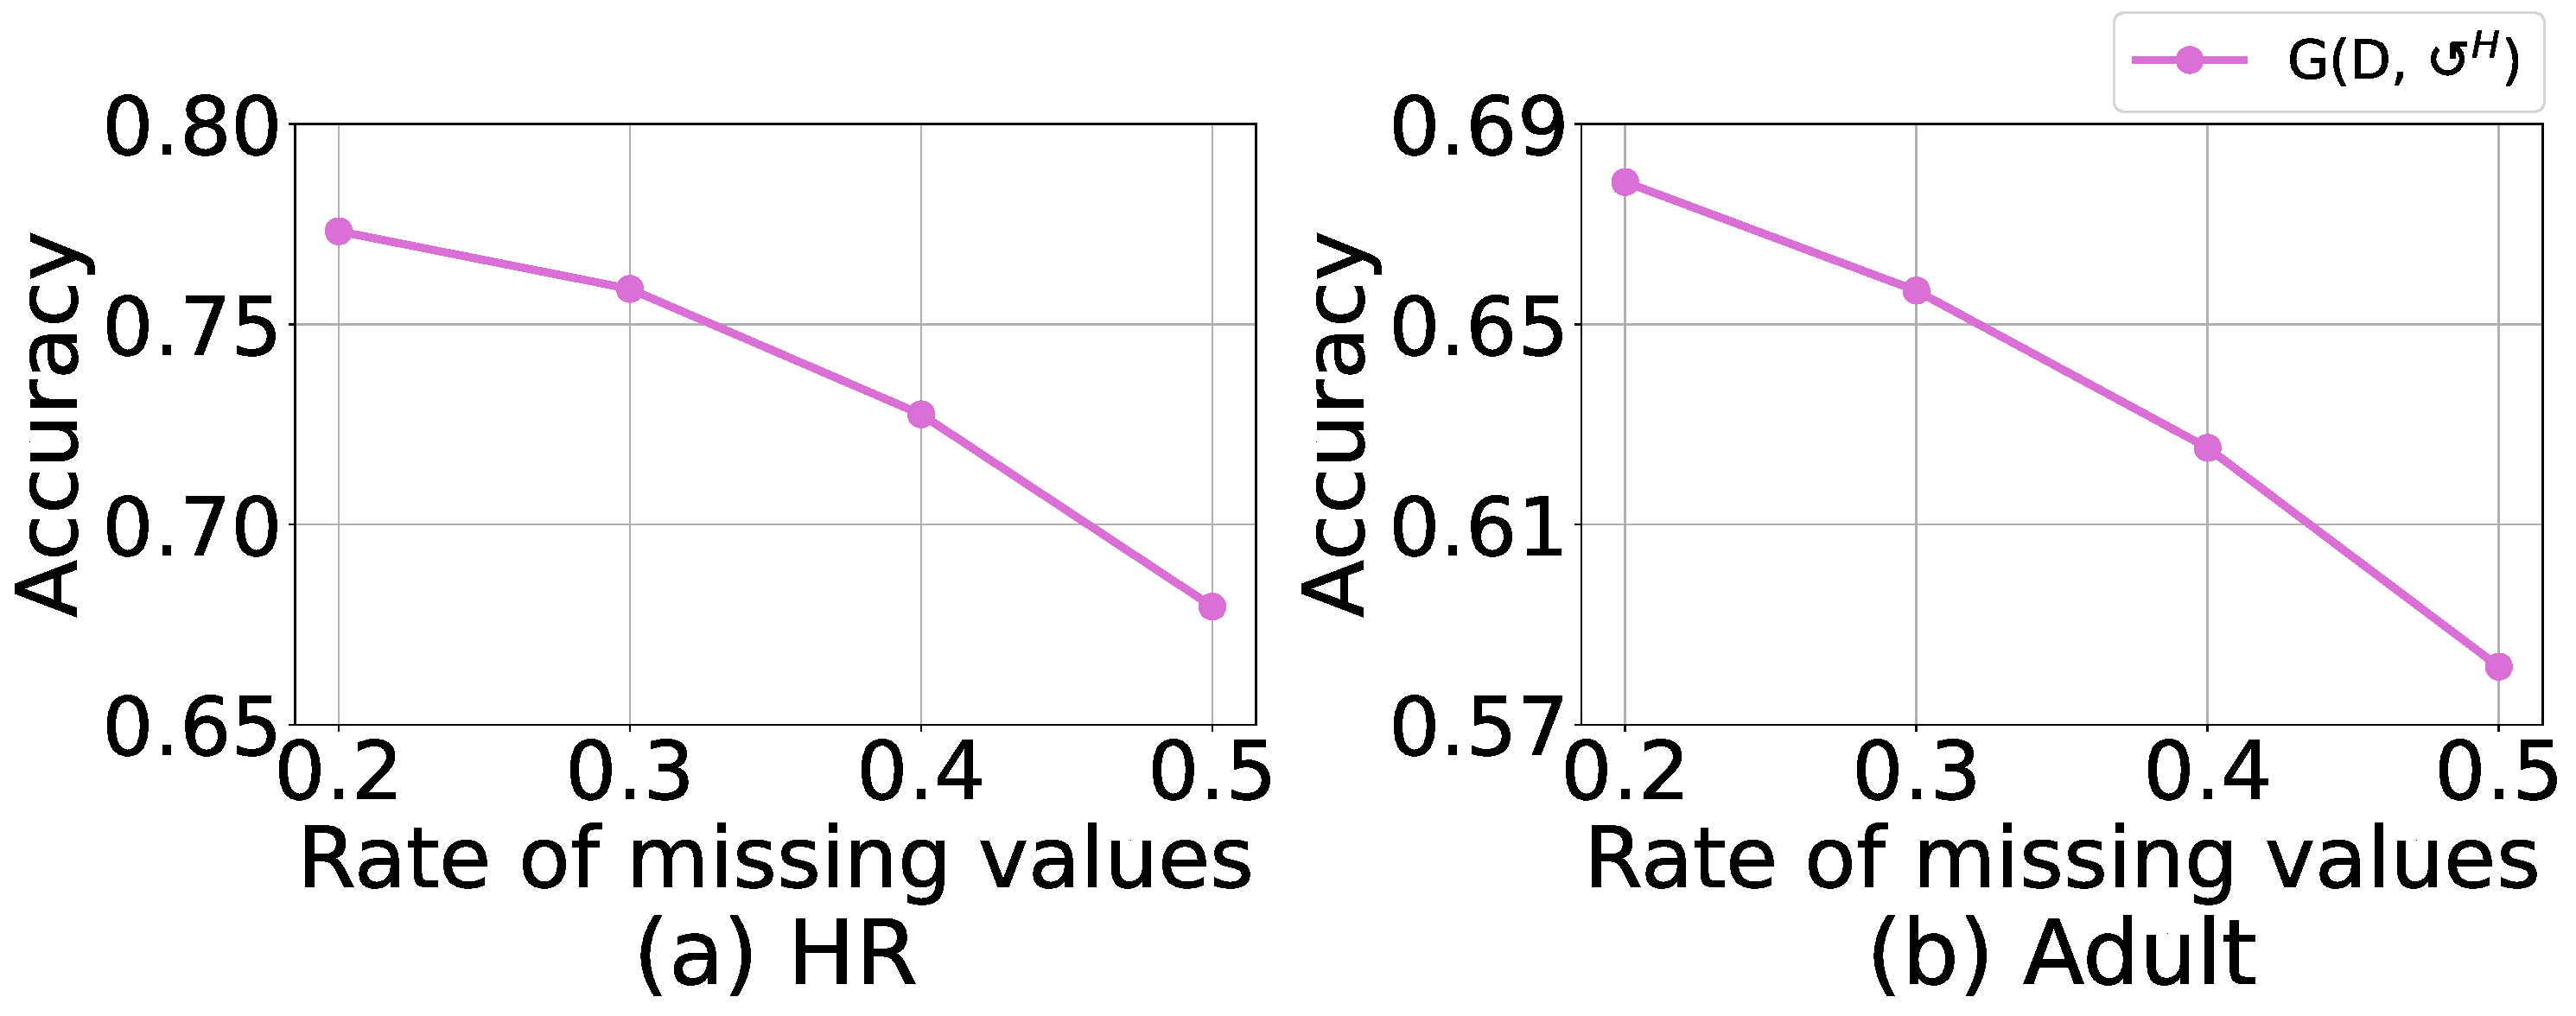
\includegraphics[width=0.5\textwidth]{figs/missingrate_real}
% %	\vspace{-1em}
% 	\caption{Varying missing value rate.}
% 	\label{fig:realmissrate}
% %	\vspace{-1em}
% \end{figure}

Recap that \ours needs the user-specified coreset size as input. Thus, we discuss how to select an appropriate coreset size. We adopt a simple yet effective solution that starts from a coreset with a small size, train over it and
evaluate via a validation set, enlarge the coreset and iteratively
train  until the performance does not improve much. 
To be specific, initially, we begin with $\rho = 10^{-4}$, and   enlarge the coreset by 2 times iteratively. If the performance on validation set varies no more than 0.5\% within three
successive iterations, we will
stop.
 Figure~\ref{fig:e2e} shows the performance on dataset \hr, \adult and \bike when varying the coreset size. We can see that the performance first improves rapidly, then remains  stable just after several iterations. For example, on dataset \adult, when $\rho=5\times 10^{-3}$, the accuracy has improved  to 72.85\% on the validation set. Empirically, an ideal coreset size is between $\rho=10^{-3}$ to $10^{-2}$.

 \begin{figure}
	\vspace{-1em}
	\centering
	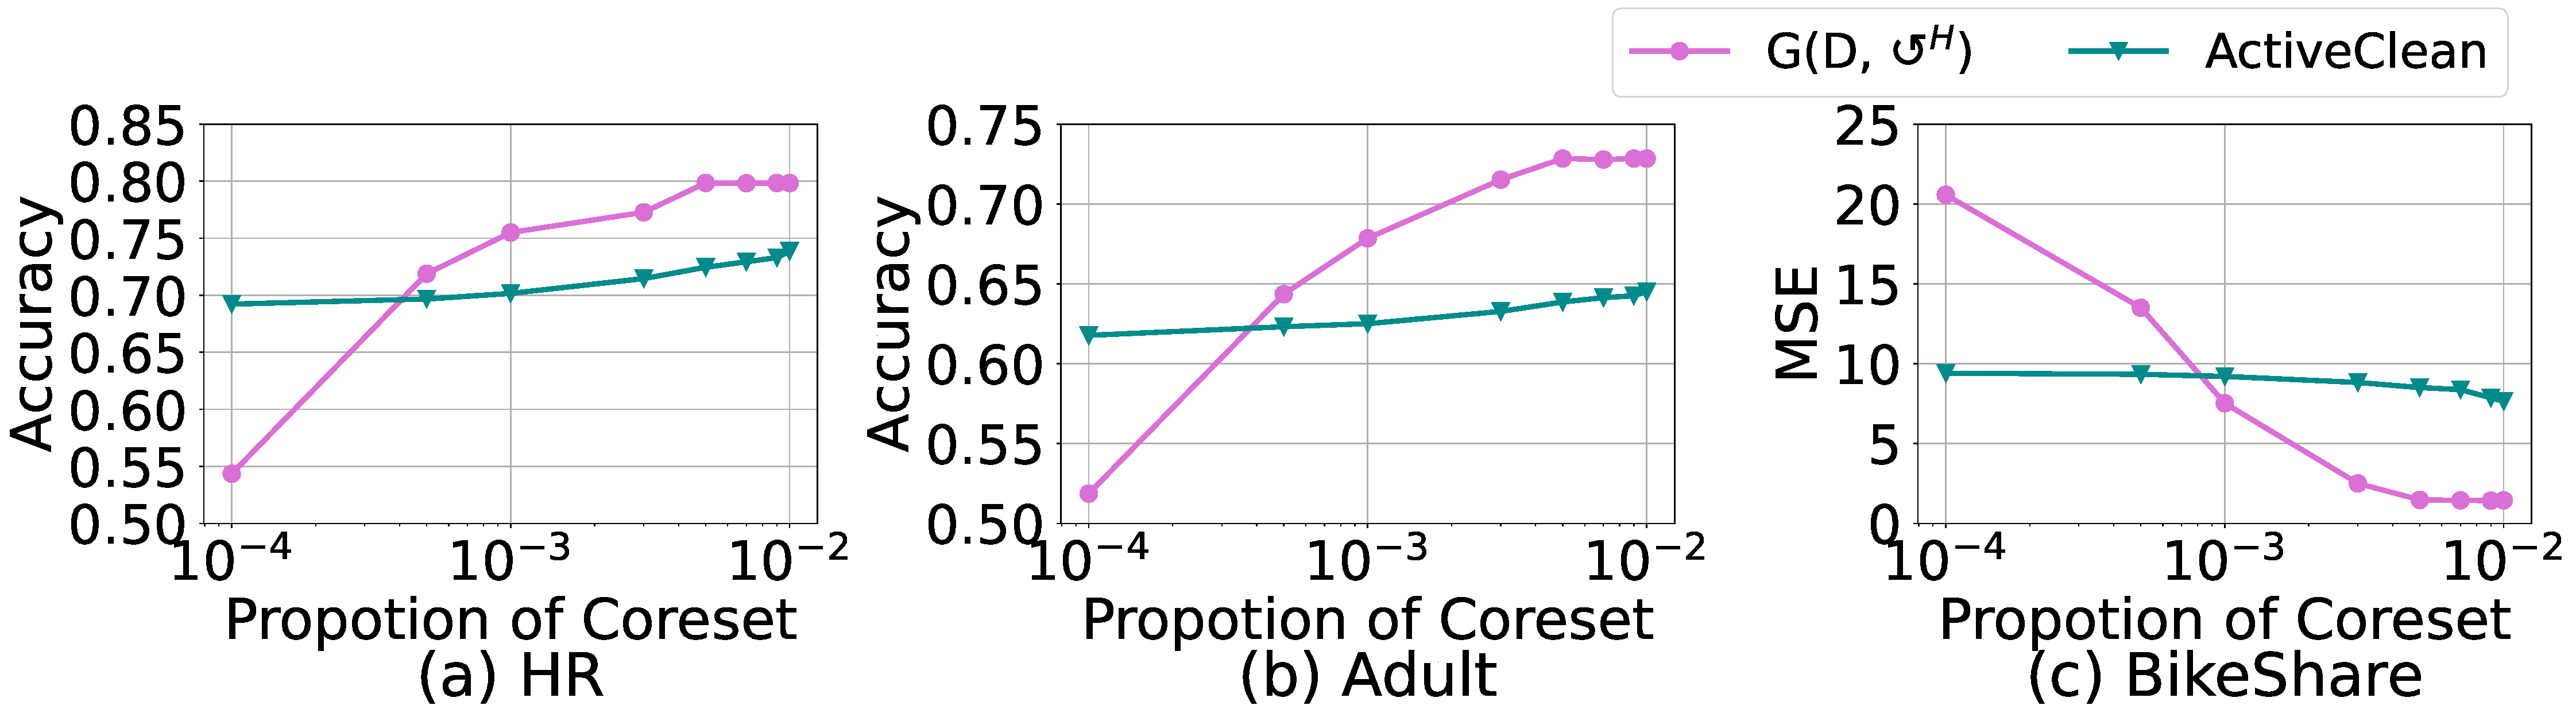
\includegraphics[width=0.8\textwidth]{figs/e2e}
%	\vspace{-2.5em}
	\caption{ Coreset size selection of \ours.}
	\label{fig:e2e}
%	\vspace{-1.8em}
\end{figure}
 
\noindent \textbf{Summary.} The results show that coreset size is not difficult to determine. If the user is willing to specify a coreset size like in Section~\ref{exp:sec:overall} based on the empirical finding, we can directly compute a coreset without training. If she cannot, we can also get a good coreset with just several training iterations over small coresets, which is also efficient.
 
\begin{figure}   
	\centering
	\begin{minipage}[t]{0.49\textwidth}
		\centering
		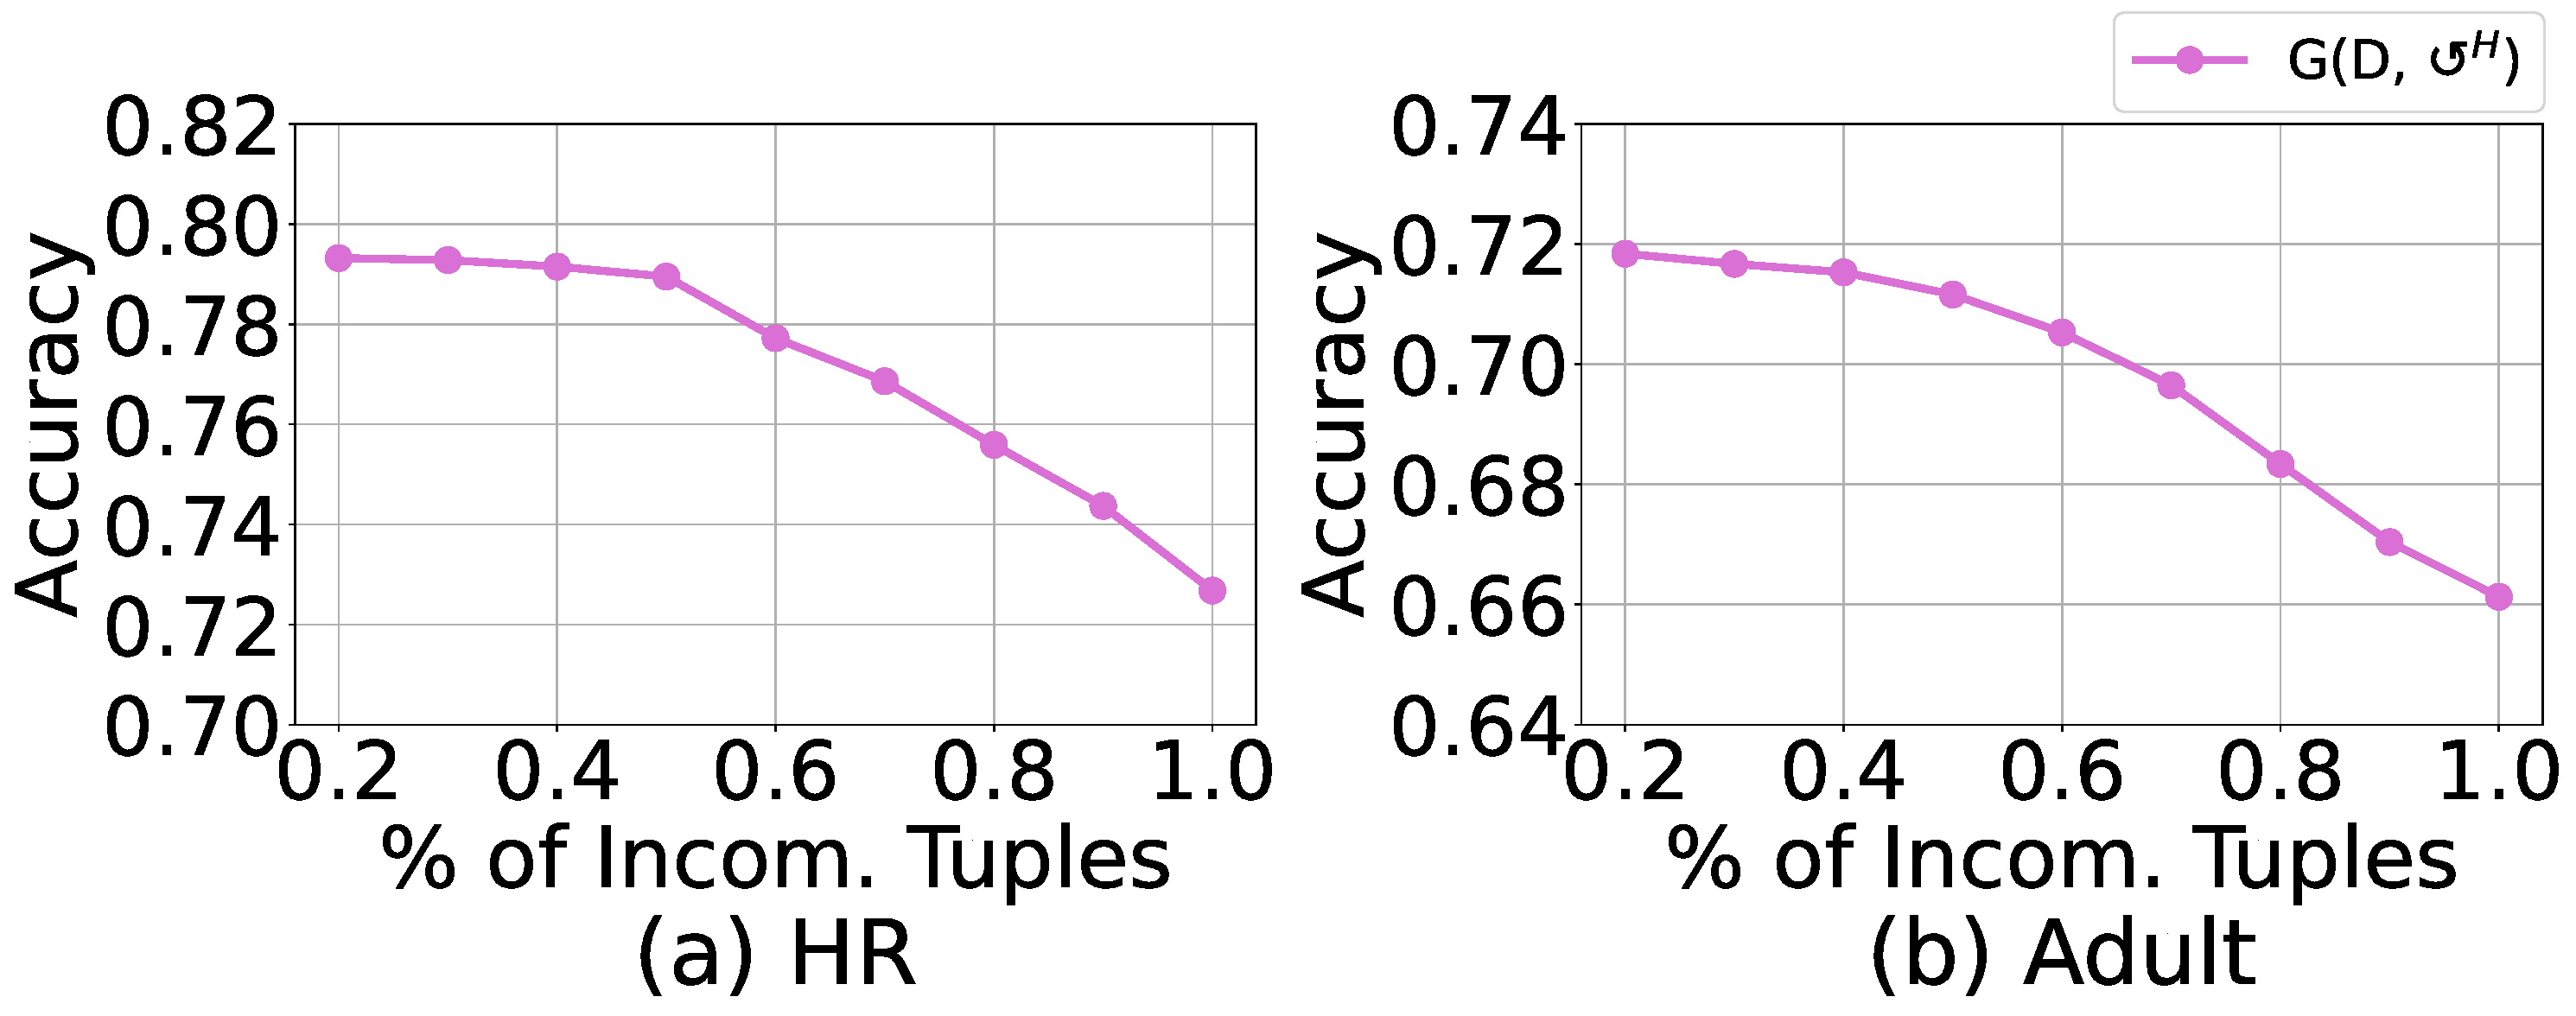
\includegraphics[width=\textwidth]{figs/missingrate_all}
    %	\vspace{-1em}
        \caption{Varying missing tuple rate.}
        \label{fig:vary_misstuple_all}
	\end{minipage}
	\begin{minipage}[t]{0.49\textwidth}
		\centering
		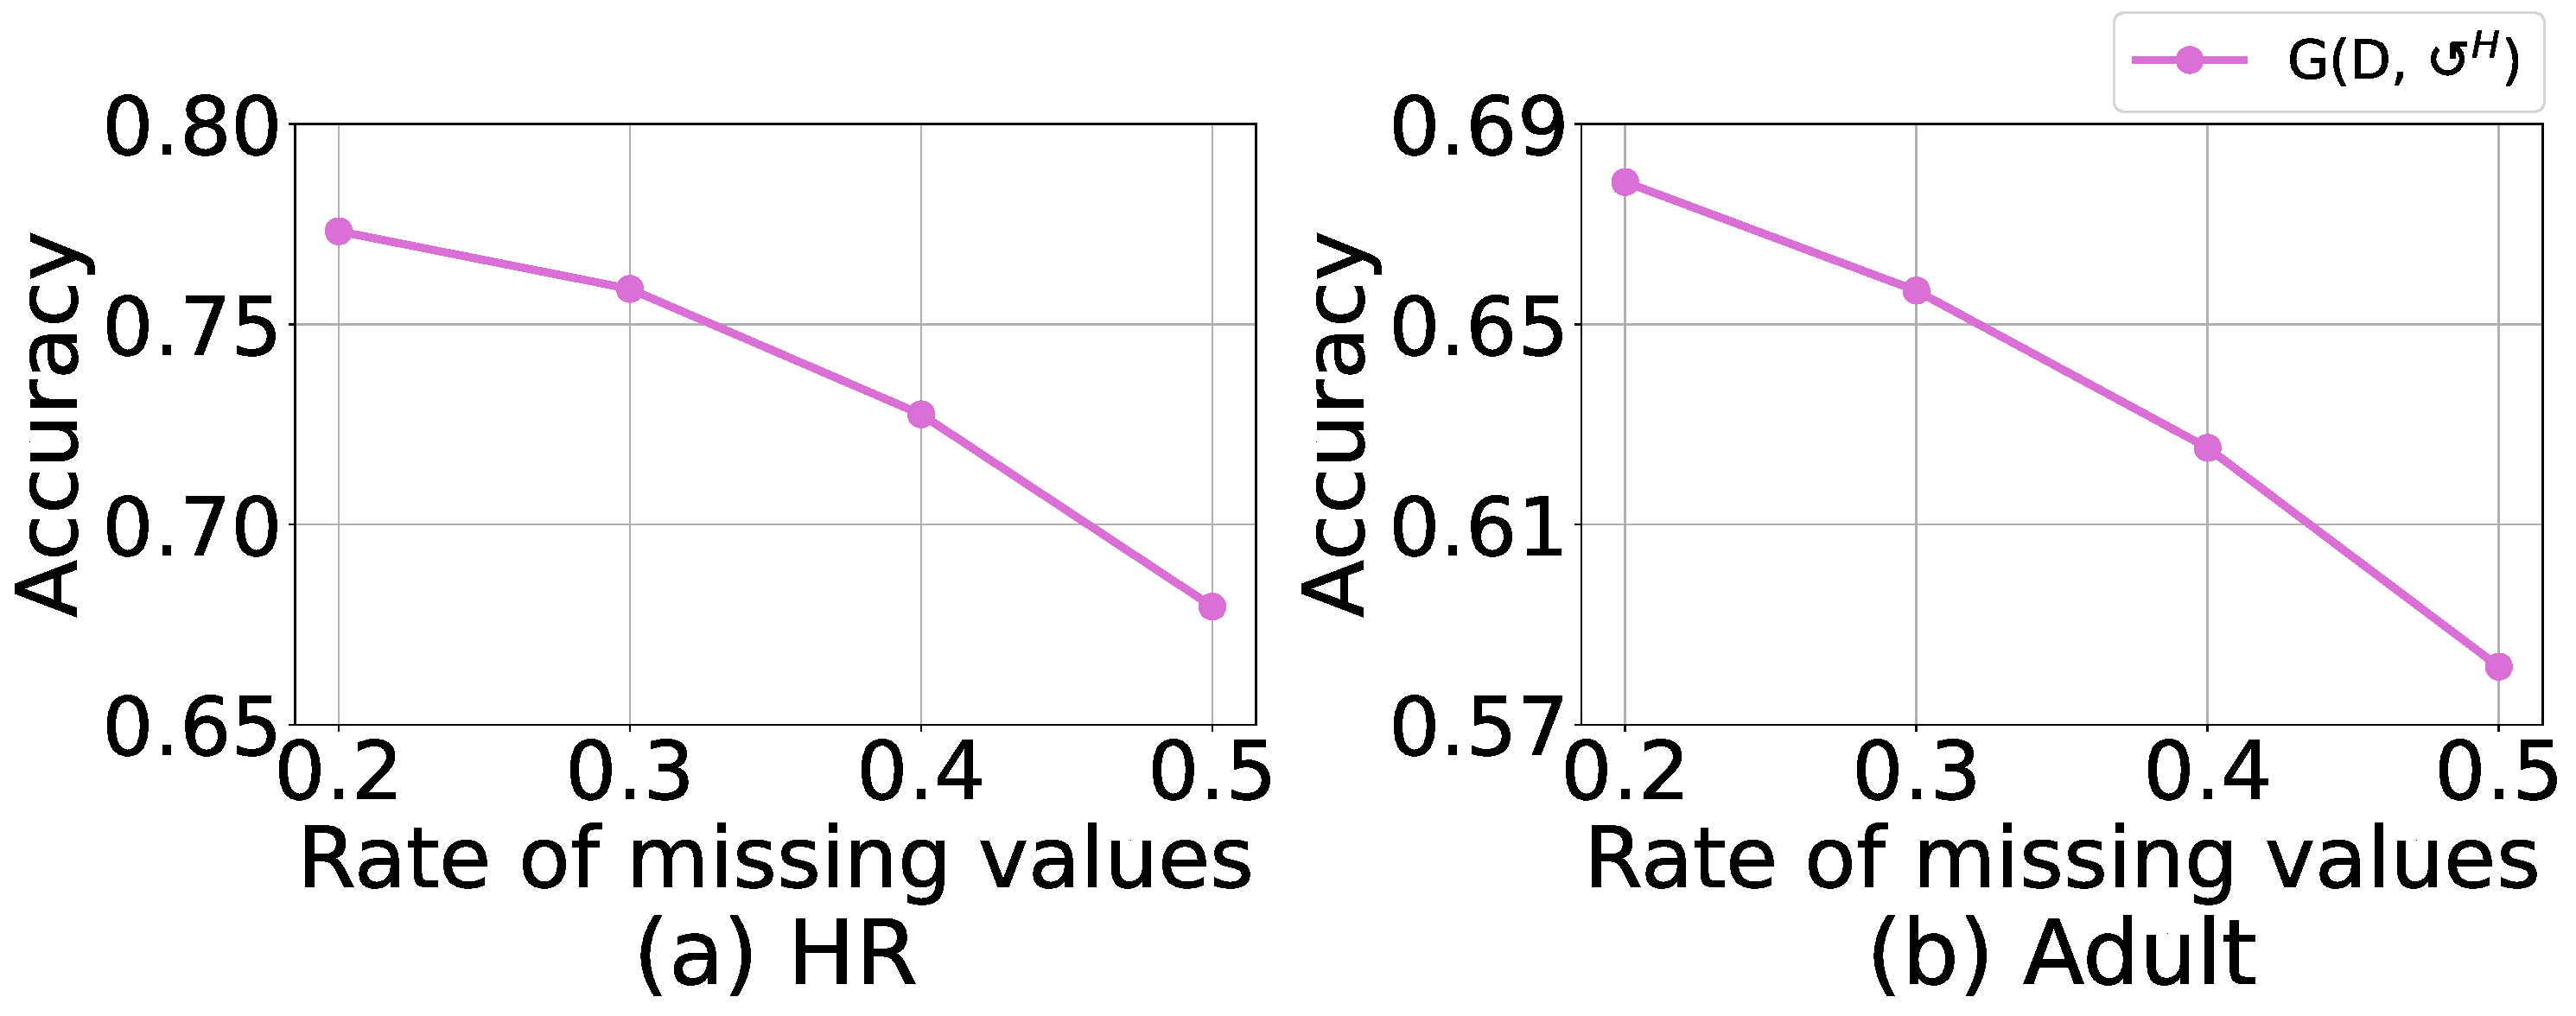
\includegraphics[width=\textwidth]{figs/missingrate_real}
    %	\vspace{-1em}
        \caption{Varying missing value rate.}
        \label{fig:realmissrate}
	\end{minipage}  
\end{figure}

\noindent{\bf Compare with \actclean.} 
Figure~\ref{fig:e2e} also reports an interesting comparison with \actclean. Specifically, 
in \actclean, we use the coreset size $K$ as the budget, i.e., number of tuples to be imputed by human in each active cleaning iteration.  
We can observe that at the beginning, when the coreset size is very small, \actclean is better because it trains with the entire dataset including the imputed tuples, while we train the model using only  few tuples in the coreset.
However, as with the increase of the coreset size, we can see that $\seven$ outperforms \actclean. This is because \actclean uses a heuristic method to estimate the impact of tuples to the overall gradient, which is not theoretically bounded (e.g., with gradient bounds like Coreset) and thus not accurate enough.
For $\seven$, it can achieve high accuracy with a proper coreset size, which is not large.











 